\documentclass{article}

\usepackage[margin=1in]{geometry}
\usepackage{graphicx}
\usepackage{amsmath}
\usepackage[colorlinks,bookmarks,bookmarksnumbered,allcolors=blue]{hyperref}
\usepackage{booktabs} % better tables
\usepackage[capitalise]{cleveref}

\begin{document}

\title{Wind Farm Optimization Case Studies
\\
\small{IEA Task 37 on System Engineering in Wind Energy}
}
\author{\small Nicholas F. Baker\thanks{Masters Student, Department of Mechanical Engineering},\  Andrew P. J. Stanley\thanks{Ph.D. Candidate, Department of Mechanical Engineering}, \ Jared Thomas\thanks{Ph.D. Student, Department of Mechanical Engineering}, \ and Andrew Ning\thanks{Assistant Professor, Department of Mechanical Engineering} \\
    {\small Brigham Young University, Provo, Utah, USA}\\
\vspace{-1em}\\
\small Katherine Dykes\thanks{Senior Engineer, National Wind Technology Center}\\
    \small National Renewable Energy Laboratory, Golden, Colorado, USA}
\maketitle

\section{Introduction}

Two major factors that affect wind farm layout optimization are 1) the optimization approach and 2) the wake model. This document defines two case studies designed to study these factors. One may elect to participate in either or both cases.
\begin{enumerate}
\item Optimization-Only Case Study: user chooses optimization approach, wake model is fixed and supplied with this study.
\item Combined Case Study: user is free to choose both optimization approach and wake model.
\end{enumerate}

Participants will optimize turbine locations to maximize annual energy production, submit solutions, and provide details on their methodology.  After all submissions are received, participants will be expected to perform a cross comparison of other participant solutions.  Data will be consolidated, processed, and made available to all participants.

\section{Problem Definition}

\subsubsection*{Objective}

The objective of each scenario is to maximize annual energy production, which we define simply as the expected value of aerodynamic power.  The wind resource for each case has a wind rose binned into 16 discrete directions, with a constant wind speed.  In other words:
\begin{equation*}
AEP = \left(\sum_{i=1}^{16} f_i P_i\right) 8760 \frac{\textrm{hrs}}{\textrm{yr}}
\end{equation*}
where $P_i$ is the power produced for wind direction $i$, and $f_i$ is the corresponding wind direction probability.

\subsubsection*{Design Variables}

The design variables are the $(x, y)$ locations of each turbine.  All locations in this document refer to the hub location.  Every turbine in the farm is identical.  

\subsubsection*{Constraints}

Each scenario has a fixed circular boundary centered at $(0, 0)$.  All turbine $(x, y)$ locations must remain on or within this boundary.  No turbine can be closer than two rotor diameters to any other turbine.

\subsubsection*{Parameters}

The wind turbine is the IEA37 3.35 MW onshore reference turbine \cite{NREL335MW} with the following characteristics:
\begin{center}
\begin{tabular}{@{}lrl@{}}
\toprule
Rotor Diameter & 130 & m \\ 
Turbine Rating & 3.35 & MW \\ 
Cut-In Wind Speed & 4 & m/s \\ 
Rated Wind Speed & 9.8 & m/s \\ 
Cut-Out Wind Speed & 25 & m/s \\
\bottomrule
\end{tabular}
\end{center}

The power curve is defined as:   

\begin{minipage}{0.5\textwidth}
\begin{equation*}
P(V) = 
\begin{cases} 
0 & V < V_{\textit{cut-in}} \\
P_{\textit{rated}}\bigg(\frac{V-V_{\textit{cut-in}}}{V_{\textit{rated}}-V_{\textit{cut-in}}}\bigg)^3 & V_{\textit{cut-in}}\leq V \leq V_{\textit{rated}} \\
P_{\textit{rated}} & V > V_{\textit{rated}}
\end{cases}
\label{eq:power}
\end{equation*}
\end{minipage}\qquad
\begin{minipage}{0.5\textwidth}
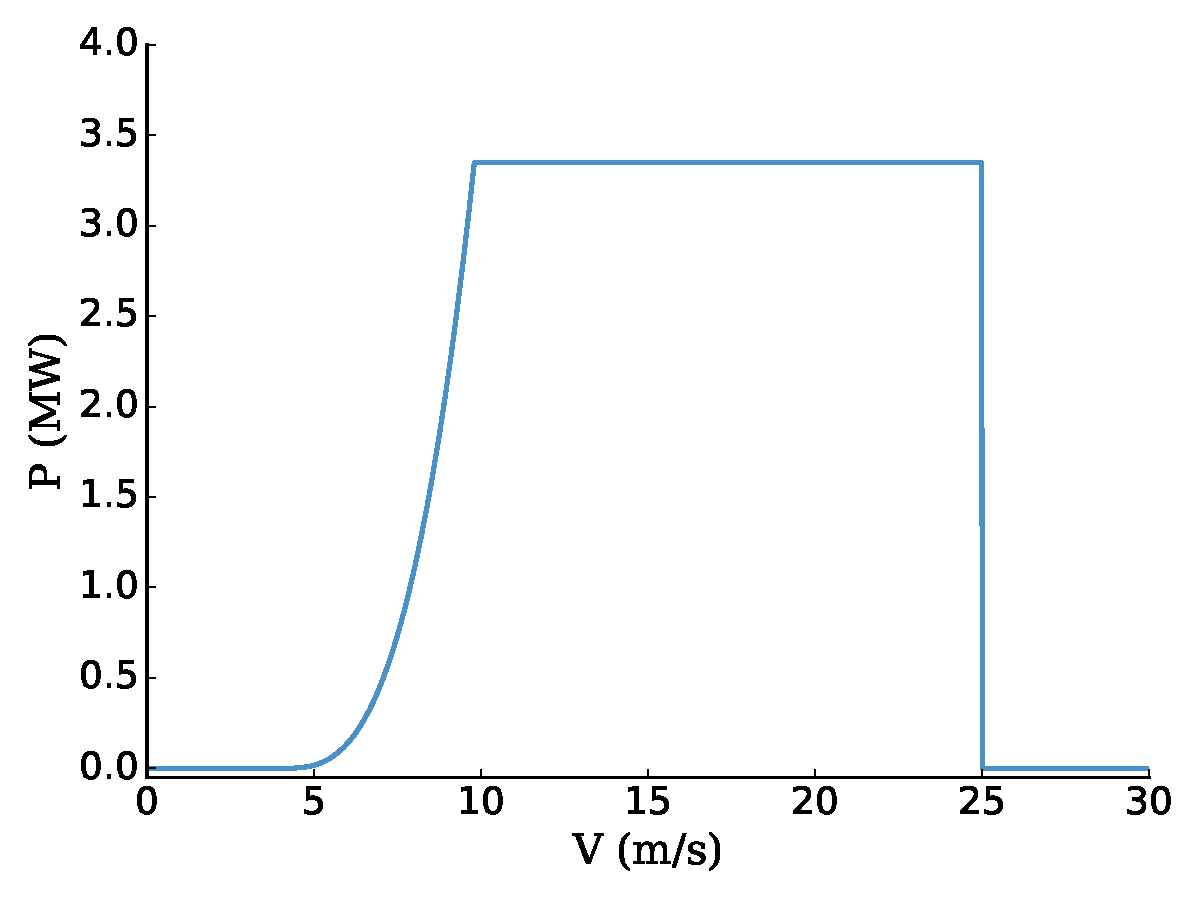
\includegraphics[width=2.5in]{power_curve}
\end{minipage}


The wind rose is defined by 16 discrete bins tabulated in baseline.yaml and depicted pictorially below.

\subsection{Optimization Only}

This problem defines three different wind farm sizes, and corresponding number of turbines, meant to test scalability of the optimization approach.  These three scenarios are:
\begin{enumerate}
    \item 16 turbines, boundary radius of 1,300 m.
    \item 36 turbines, boundary radius of 2,000 m.
    \item 64 turbines, boundary radius of 3,400 m.
\end{enumerate}

The user is only free to choose the optimization approach.  The wake model for this study is fixed and is a version of Bastankhah's Gaussian wake model \cite{Thomas2018, Bastankhah2014, Bastankhah2016}.  A Python implementation is supplied for convenience (AEPcalc.py). Alterations to the implementation are permitted, as long as the governing physics equations are not altered.  Participants may use other programming languages, but must use the same physics equations.  To aid with this, the relevant equations are defined in a separate document (wake-model.pdf), and example layouts with corresponding AEP values are provided in (example.yaml) to verify implementations.  The example designs are only for verification, and do not need to be used as starting points in your optimization.  

\subsection{Combined}

This problem defines one scenario where the user is free to choose both the optimization algorithm and the wake model.  The wind farm contains nine turbines with a boundary radius of 900 m.  If needed by the wake model, the turbulence intensity is 0.75, and the wind shear is a power-law with a shear exponent of 0.15 using the hub height as the reference height.

\section{Reporting and Evaluation}

Participants will submit:
\begin{enumerate}
    \item optimal solution for each scenario using the format in example.yaml 
    \item a survey describing the methodology and simulation environment \url{here}.
\end{enumerate}

\subsection{Optimization Only}

Results will be compared by running AEPcalc.py using the provided yaml file from each participant.  Uses must adhere to the format in order to receive a ranking.  While other implementations may be used in the optimization, all evaluations will be done with the provided AEPcalc.py code so it is essential that you check that your implementation is consistent.

\subsection{Combined}

Because the wake models differ in this case, determining a ``best'' solution is generally not possible.  Comparisons will be made using two approaches:
\begin{enumerate}
    \item Every participant will evaluate every other participant's solutions using their own wake models.  It is essential that the yaml format is adhered to so that cross-comparisons are painless.  If the optimizations behave as expected than each participant will judge their own solution as best, but it is possible that a solution is found that other wake models agree is better.
    \item Each solution will be compared using a higher-fidelity simulation, in this case large-eddy simulations using SOWFA.  This introduces its own modeling assumptions and is an imperfect way to compare, but does provide another piece of information on relative performance between solutions.  It is expected that solutions with minor LES performance differences would lie within the error of the methodology and thus only major differences would be used in drawing conclusions on relative performance.
\end{enumerate}


\bibliographystyle{aiaa}
\bibliography{references}

\end{document}